\section{Galois Group}
Let \(F\) be a field. ``The set \(AutF\) of all field-automorphisms \(F \rightarrow F \) forms a group under the function composition'' \cite{hunger}.\\[3mm]
\noindent
Let \(E\) and \(F\) be the extension fields of a field \(K\).\\
If a non-zero field-homomorphism \(\sigma : E \rightarrow F\) is a K-module homomorphism then\\
\(\sigma(k)=\sigma(k1_E)=k\sigma(1_E)=k1_F=k\).\hspace{7mm}
i.e, \(\sigma\) fixes \(K\) element-wise.\\
Conversely, if a field homomorphism \(\sigma : E \rightarrow F\) fixes K element-wise, then \(\sigma\) is a non-zero and for any \(u \in E\), we have, \(\sigma(ku)=\sigma(k)\sigma(u)=k\sigma(u)\)
i.e \(\sigma\) is a K-module homomorphism \cite{hunger}.
\begin{definition} \cite{hunger}
  A field-automorphism \(\sigma \in Aut F\) which is also K-homomorphism is called K-automorphism. In other words, a field-automorphism \(\sigma \in Aut F\) that fixes K element-wise is called K-automorphism.
\end{definition}

\begin{definition} \cite{hunger}
  The group of all K-automorphisms of \(F\) is called the Galois group of \(F\) over \(K\) and it is denoted by \(Aut_K^F\).
\end{definition}

\section{Galois extension}
Let \(E\) be an intermediate field and \(H\) be a subgroup of \(Aut_K^F\), then:
\begin{enumerate}
\item[i)] ``\(H' = \{v \in F \; | \: \sigma(v)=v,\) for all \(\sigma \in H \}\)'' \cite{hunger} is an intermediate field of the extension field \(F\) of \(K\);
\item[ii)] ``\(E' = \{\sigma \in Aut_K^F \; | \; \sigma(u)=u,\) for all \(u \in E\}=Aut_E^F\)'' \cite{hunger} is a subgroup of \(Aut_K^F\).
\end{enumerate}

The field \(H'\) is called the fixed field of the subgroup H in F \cite{hunger}.

\subsection{Fixed Field}
We have,\\
\(H' \rightarrow\) fixed field and \(E' \rightarrow\) \(Aut_E^F\).\hspace{5mm} Let \(Aut_K^F = G\) then the field fixed by it is \(G'\). It is not necessary that the field fixed by \(G\) is \(K\) i.e, \(G'=K\).
\vspace{3mm}
\begin{example}
  For \(f(x)=x^3-2 \in Q[x]\). Let \(u \in F\) such that \(f(u)=0\) and let \(F=Q[u]\).Then
  \(G=Aut_Q^{Q(u)}={1}\) so, \hspace{5mm}\(G'=F \neq K\).
\end{example}

\vspace{3mm}
\begin{definition} \cite{hunger}
Let \(F\) be an extension field of \(K\) such that the fixed field of the Galois group \(Aut_k^F\) is \(K\) itself. Then \(F\) is said to be a Galois extension of \(K\) or Galois over K.
\end{definition}

\section{Fundamental Theorem of Galois Theory}
\begin{tcolorbox}
\begin{theorem} \cite{hunger}
  If \(F\) is a finite dimensional Galois extension of \(K\), then there is a one-to-one correspondence between the set of all intermediate fields of \(F\) over \(K\) and the set of subgroups of the Galois group \(Aut_K^F\) such that:
  \begin{enumerate}
  \item[i)] the relative dimension of two intermediate fields is equal to the relative index of the corresponding subgroups. In particular \(Aut_K^F\) has order \([F:K]\);
  \item[ii)] \(F\) is Galois over every intermediate field \(E\), but \(E\) is Galois over \(K\) if and only if the corresponding subgroup \(E'= Aut_E^F\) is normal in \(G=Aut_K^F\).In this case \(G/E'\) is isomorphic to the Galois group \(Aut_K^E\) of \(E\) over \(K\).
  \end{enumerate}
\end{theorem}
\end{tcolorbox}

\vspace{2mm}
We already have a correspondence between the intermediate fields and the subgroup of Galois group.\\
That is to each intermediate field \(E\), there is a subgroup \(Aut_E^F\) and to each subgroup \(H\) there is a fixed field \(H'\). But this correspondence is one-to-one if and only if for each intermediate field \(E\), it satisfies \(E''=E\) and for each subgroup \(H\), it satisfies \(H''=H\).

\subsection{Closed Field and Subgroup}
\begin{definition} \cite{hunger}
  Let \(X\) be an intermediate field or subgroup of the Galois group. \(X\) will be called \textbf{closed} provided \(X=X''\).
\end{definition}
\clearpage

\begin{lemma} \cite{hunger}
\begin{enumerate}
\item[i)] If \(F\) is an extension field of \(K\), then there is one-to-one correspondence between the closed intermediate fields of the extension and the closed subgroups of the Galois group, given by \(E \rightarrow E' =  Aut_E^F\).
\item[ii)] If \(F\) is a finite dimensional Galois extension of \(K\), then all intermediate fields and all subgroups of the Galois group are closed and \(Aut_K^F\) has order \([F:K]\).
  \end{enumerate}
\end{lemma}
\vspace{3mm}

\subsection{Stable Intermediate}
\begin{definition} \cite{hunger}
  An intermediate field \(E\) of \(F\) over \(K\) is said to be stable intermediate if \(\sigma(E) \subseteq E\) for every \(\sigma \in Aut_K^F\) .
\end{definition}

\begin{lemma} \cite{hunger}
  \begin{enumerate}
  \item[i)] If E is a stable intermediate field of the extension, then \(E'=Aut_E^F\) is a normal subgroup of the Galois group \(Aut_K^F\) ;

  \item[ii)] if \(H\) is a normal subgroup of \(Aut_K^F\), then the fixed field \(H'\) of \(H\) is a stable intermediate field of the extension
  \end{enumerate}
\end{lemma}
\vspace{3mm}

\subsection{Proof of the Fundamental Theorem}
\begin{proof}
From lemma 1 above, one-to-one correspondence between the intermediate fields and the subgroups follows \cite{hunger}. And from lemma 2 the next two statements of the theorem follows \cite{hunger}.
\end{proof}
\vspace{3mm}

\section{Application}
The fundamental theorem links Field theory to Group theory. This allows us to use the tools of Group theory to solve the problems involving field theory. Solving a polynomial equation is a problem of field theory. We can use insights of Group theory to solve this problem of field theory which is discussed in some detail in next part of this thesis \cite{hunger}.
\clearpage

\section{Illustration of The Fundamental Theorem}
\begin{minipage}{0.68\textwidth}
  Let \(F\) be an Galois extension of a field \(K\). Let the towers of the intermediate fields of \(F\) over \(K\) be as follows:
  \[
    K \subset E \subset F
  \]
\noindent
  Let \(G\) be the Galois group of \(F\) over \(K\). Then its subsets are
  \[
    \{e\} \subset H \subset G
  \]
  Then the one-to-one correspondence is as shown:
\end{minipage}\hspace{2mm}
\begin{minipage}{0.3\textwidth}

  \begin{tcolorbox}[colback=gray!20, colframe=blue!20, title={\footnotesize \textcolor{black}{Galois-correspondence}}, width=5cm]
    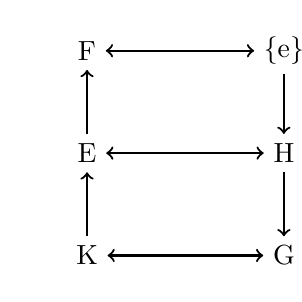
\begin{tikzpicture}
      \hspace{5mm}
      \node (f) {F};
      \node[below of=f, yshift=-3mm] (e) {E};
      \node[below of=e, yshift=-3mm] (k) {K};

      \draw[<-,thick] (f)--(e);
      \draw[<-,thick] (e)--(k);

      \node[right of=f, xshift=15mm] (i) {\{e\}};
      \node[below of=i, yshift=-3mm] (h) {H};
      \node[below of=h, yshift=-3mm] (g) {G};

      \draw[->, thick] (i)--(h);
      \draw[->, thick] (h)--(g);

      \draw[<->, thick] (f)--(i);
      \draw[<->, thick] (e)--(h);
      \draw[<->, thick] (k)--(g);
    \end{tikzpicture}
  \end{tcolorbox}
\end{minipage}

\vspace{5mm}
\begin{remark}
  The intermediate fields are getting larger as we go from bottom to top as the fields are getting extended. But the subgroups are getting smaller.
\end{remark}

\vspace{7mm}
\section{Insights to the Fundamental Theorem}

\subsection{Nature of a Number}
\textcolor{blue}{The nature of a number depends upon the underlying field.} \\
\(\sigma:\{a+b\sqrt{2}\} \mapsto \{a-b\sqrt{2}\}\) where \(a,b \in \mathbb{Q}\) is a field-automorphism of  \(\mathbb{Q}(\sqrt{2})\) that fixes \(\mathbb{Q}\). This map \(\sigma \) is also denoted by \(\sqrt{2} \longmapsto -\sqrt{2}\). So, any polynomial equation over \(\mathbb{Q}\) satisfied by the number \(\sqrt{2}\) is also satisfied by the number \(-\sqrt{2}\). You can fluidly pass between these two numbers and the equation with a rational coefficient will not know. \textit{Hence the two numbers \(\sqrt{2}\) and \(-\sqrt{2}\) are algebraically same over \(\mathbb{Q}\).}\\

But the map \(\sqrt{2} \longmapsto -\sqrt{2}\) does not fix the field \(\mathbb{Q}(\sqrt{2})\) i.e does not fix itself. The only automorphism of \(\mathbb{Q}(\sqrt{2})\) is the identity map. So, you cannot pass \(\sqrt{2}\) for \(-\sqrt{2}\) for every equation with coefficients in \(\mathbb{Q}(\sqrt{2})\). \textit{Hence the two numbers \(\sqrt{2}\) and \(-\sqrt{2}\) are not algebraically same over \(\mathbb{Q}(\sqrt{2})\).}
\vspace{7mm}

\begin{figure}[h]
  \centering
 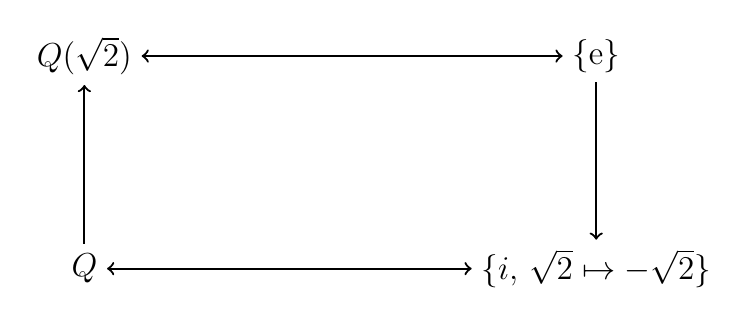
\begin{tikzpicture}
      \node (f) {\large \(\mathbb{Q}(\sqrt{2})\)};
      \node[below of=f, yshift=-17mm] (e) {\large \(\mathbb{Q}\)};


      \draw[<-,thick] (f)--(e);

      \node[right of=f, xshift=55mm] (i) {\large \{e\}};
      \node[below of=i, yshift=-17mm] (h) {\large \{\(i\), \(\sqrt{2} \mapsto -\sqrt{2}\)\}};


      \draw[->, thick] (i)--(h);


      \draw[<->, thick] (f)--(i);
      \draw[<->, thick] (e)--(h);
    \end{tikzpicture}
    \end{figure}
\clearpage

\subsection{Structure of a Field}
The structure of a field as an extension field over some field is mirrored in the structure of the ``group'' of  permutations of its elements that keeps the base field fixed. But these permutations are the symmetries of the field. \textit{So, the structure of field extension is equals to its own symmetry.}\\

The structure of a field is a \textbf{complicated} thing; specially if it is infinite. But the structure of a group is rather simple; especially if it is finite. So the Galois theory has fairly simplified the complicated thing in a very insightful and beautiful way.\\

Also Galois theory gives a new sights of study of fields which is ``study of fields via study of its automorphisms'' which are permutations of the field. That is\\[5mm]

\begin{figure}[h]
  \centering
  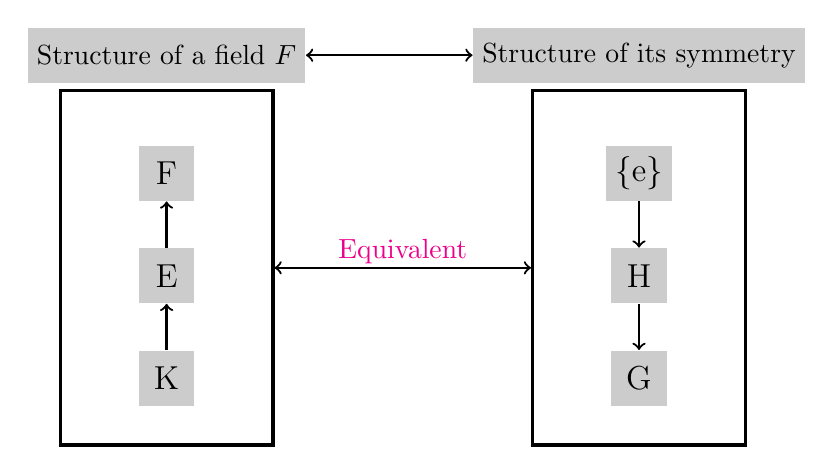
\begin{tikzpicture}

    \node[rectangle, very thick, draw,
    minimum height=4.5cm,
    minimum width=2.7cm] (rec) at (0,0) {};

    \node[rectangle, very thick, draw,
    minimum height=4.5cm,
    minimum width=2.7cm] (rec2) at (6,0) {};


    \node[minimum width=7mm,
      minimum height=7mm,
      fill=gray!40,
      ] (ss) at (0,2.7) {Structure of a field \(F\)};

      \node[minimum width=7mm,
      minimum height=7mm,
      fill=gray!40,
      ] (ss2) at (6,2.7) {Structure of its symmetry};

      \draw[<->, thick] (ss)--(ss2);
       \draw[<->, thick] (rec)--(rec2);

      \node[minimum width=7mm,
      minimum height=7mm,
      fill=gray!40] (f) at (0,1.2) {\large F};

      \node[minimum width=7mm,
      minimum height=7mm,
      fill=gray!40,
      below of=f, yshift=-3mm] (e) {\large E};

      \node[right of=e,
      xshift=20mm, yshift=3mm] (txt) {\textcolor{magenta}{Equivalent}};

      \node[minimum width=7mm,
      minimum height=7mm,
      fill=gray!40,
      below of=e, yshift=-3mm] (k) {\large K};

      \draw[<-,thick] (f)--(e);
      \draw[<-,thick] (e)--(k);

      \node[right of=f,
      xshift=5cm,
      minimum width=7mm,
      minimum height=7mm,
      fill=gray!40,
      ] (i) {\large \{e\}};

      \node[minimum width=7mm,
      minimum height=7mm,
      fill=gray!40,
      below of=i, yshift=-3mm] (h) {\large H};

      \node[
      minimum width=7mm,
      minimum height=7mm,
      fill=gray!40,
      below of=h, yshift=-3mm] (g) {\large G};

      \draw[->, thick] (i)--(h);
      \draw[->, thick] (h)--(g);
    \end{tikzpicture}
    \caption{\footnotesize Equivalency}
\end{figure}
